\documentclass[12pt]{article}
\usepackage{comment}
\usepackage[utf8]{inputenc}
\usepackage{xspace}
\usepackage{gastex}
\usepackage{amsmath}
\usepackage{amssymb}
\usepackage{wrapfig}
\usepackage{tikz}
\usepackage{float}
\usepackage{pgfplots}
\usepackage{booktabs} % For \toprule, \midrule and \bottomrule
\usepackage{pgfplotstable} % Generates table from .csvi
\usepackage{csquotes}
\usepackage{graphicx}
\usepackage{amsmath}
\usepackage{multicol}
\usepackage{tgtermes} % times font
\usepackage[shortlabels]{enumitem}
\usepackage{parskip}

\pagestyle{empty}
\textwidth      165mm
\textheight     252mm
\topmargin      -18mm
\oddsidemargin  -2mm
\evensidemargin -2mm
% \renewcommand{\baselinestretch}{0.96}
\newcommand{\impl}{\mathbin{\Rightarrow}}
\newcommand{\biim}{\mathbin{\Leftrightarrow}}
\newcommand{\id}[1]{\mbox{\textit{#1}}}
\newcommand{\tuple}[1]{\langle #1 \rangle}
\newcommand{\ma}{\mathsf{a}}
\newcommand{\mb}{\mathsf{b}}
\newcommand{\mc}{\mathsf{c}}
\newcommand{\md}{\mathsf{d}}
\newcommand{\nat}{\mathbb{N}}
\newcommand{\intg}{\mathbb{Z}}

\newcounter{question}
\newcommand{\question}[1]{
    \stepcounter{question}
    \thequestion. #1 \hfill
}

\newcommand{\revision}[1]{
    \stepcounter{question}
    \thequestion. #1* \hfill
}



\begin{document}
\topskip0pt
\begin{center}
    {\sc The University of Melbourne
        \\
        School of Computing and Information Systems
        \\
    COMP90020 Distributed Algorithms}
    \bigskip \\
    {\Large\bf Quiz 1: Time, Ordering and Global States}
    \bigskip \\
\end{center}


\section*{Solutions}

\setcounter{question}{0}

\question{Consider a hardware clock $H(t)$ with a maximum drift rate of 0.3 seconds/second. Assume the clock is used to measure the time interval between $t=10:50:00$ and $t'=10:50:50$. What are the minimum and maximum values that can be obtained for the given time interval when measured using $H(T)$?}

\begin{enumerate}[(a)]
    \item minimum = 0.5 seconds, maximum = 1.5 seconds
    \item minimum = 25 seconds, maximum = 75 seconds
    \item They can't be determined, the roundtrip time needs to be known to estimate these values
    \item minimum = 35 seconds, maximum = 65 seconds
\end{enumerate}

\question{Consider two asynchronous distributed systems $AS_1$ and $AS_2$. Cristian's algorithm is used in both systems to synchronize clocks. In $AS_1$, the minimum transmission delay $T_{min}$ is estimated to be 0.3 seconds and process $p_1$ records a round trip time $T_{round}$ of 1.6 seconds. In $AS_2$, $T_{min}$ is estimated to be 1.2 seconds and $p_2$ records a round trip time of 2.8 seconds. Which process can achieve a higher accuracy? Explain your answer.}

\question{In the Berkely algorithm for clock synchronization, the master sends the amount by which each clock requires adjustment, as opposed to the current timestamp of the estimated average clock. This is done to: }
\begin{enumerate}[(a)]
    \item Ensure the monotonicity condition is preserved
    \item Avoid introducing further uncertainty due to message transmission delays
    \item Reduce the amount of bandwidth used by sending smaller messages
    \item Reduce the number of computations made by slaves when updating their clocks
\end{enumerate}

\question{Give an example where $a$ and $b$ are concurrent events, yet the Lamport timestamp of $a$ is smaller than the Lamport timestamp of $b$, that is, $L(a) < L(b)$.}


\question{What shortcoming of Lamport clocks do Vector clocks overcome?}

\question{Which set of events is concurrent?}
\begin{enumerate}[(a)]
    \item $[1,2,3], [3,2,4]$
    \item $[1,0,3], [2,1,1]$
    \item $[1,1,1], [2,2,2]$
    \item $[1,1,1], [1,1,1]$
\end{enumerate}

\question{Consider the figure below showing three processes $P_1, P_2, P_3$.  }

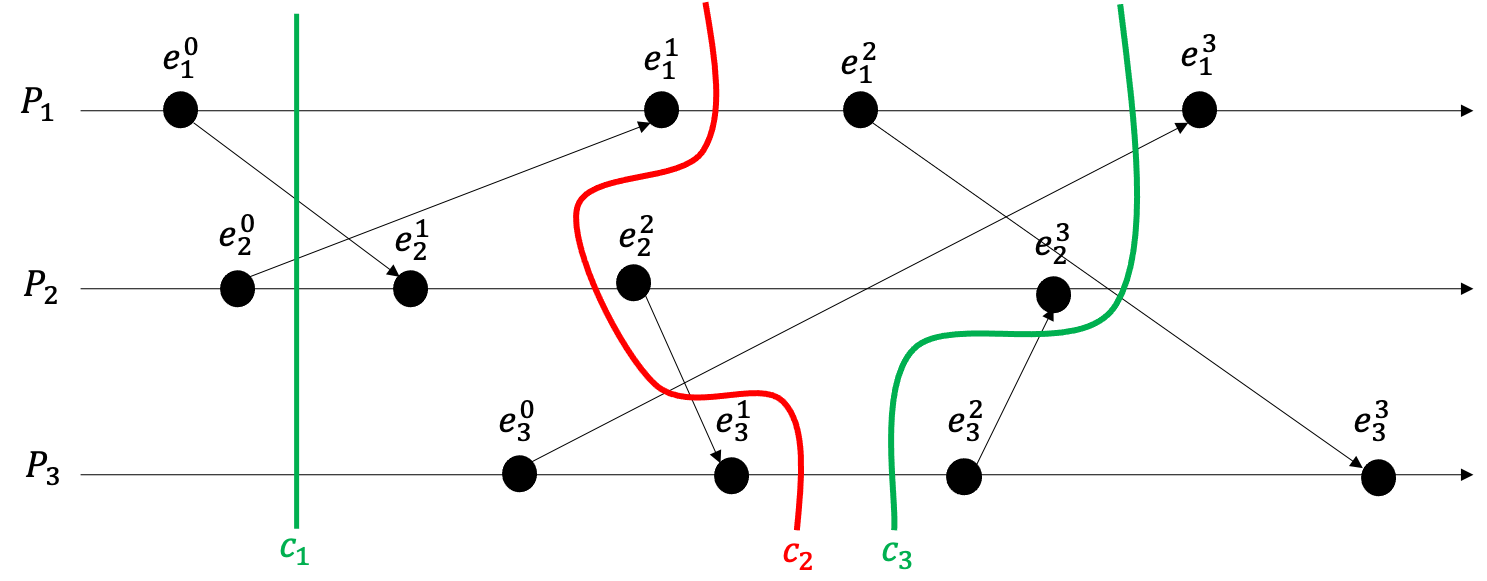
\includegraphics[scale=0.7]{cuts.png}

\begin{enumerate}[7.1]
    \item Give an example of a run that is not a linearization. Explain your answer.
    \item Is the cut, shown by curve $c_2$ (red), a consistent cut? Explain your answer.
    \item Is the state associated with $c_3$ (green) reachable from the state associated with $c_1$ (green)? Explain your answer.
\end{enumerate}

\question{With an example, show that the Chandy-Lamport algorithm will not record a consistent global state if channels are not FIFO.}

\end{document}
